\documentclass[a4paper,12pt]{article}
\usepackage[russian]{babel}
\usepackage[utf8]{inputenc}
\usepackage[hidelinks]{hyperref}
\usepackage{amssymb}
\usepackage{amsmath}
\usepackage{graphicx}
\graphicspath{{/}}
\DeclareGraphicsExtensions{.pdf,.png,.jpg}

\begin{document}
\section*{17. Способы борьбы с переобучением. Байесовская сеть доверия: определение и применение. Уменьшение размерности пространства признаков.}

\url{http://logic.pdmi.ras.ru/csclub/sites/default/files/slides/20080330_machine_learning_nikolenko_lecture07.pdf}

\url{http://www.habarov.spb.ru/new_es/exp_sys/es06/es6.htm}

\subsection*{Способы борьбы с переобучением}
Минимизацию эмпирического риска следует применять с известной долей осторожности. 
Если минимум функционала $Q(a,X^l)$ достигается на алгоритме $a$, то это ещё не гарантирует, что $a$ будет хорошо приближать 
целевую зависимость на произвольной контрольной выборке $X^k = (x_i, y_i )^k_{i=1}$.
Когда качество работы алгоритма на новых объектах, не вошедших в состав обучения, оказывается существенно хуже, чем на обучающей выборке, 
говорят об эффекте переобучения (overtraining).

Избавиться от него нельзя. Как его минимизировать?
\begin{itemize}
    \item минимизировать одну из теоретических оценок;
    \item накладывать ограничения на $\Sigma$ (регуляризация);
    \item минимизировать HoldOut, LOO или CV
\end{itemize}

Читать: 
\url{http://www.machinelearning.ru/wiki/images/6/6d/Voron-ML-1.pdf}

\url{http://www.machinelearning.ru/wiki/images/2/2d/Voron-ML-Modeling.pdf}

\subsection*{Байесовская сеть доверия}
\textit{Байесовская сеть} -- графическая вероятностная модель, представляющая собой множество переменных и их вероятностных зависимостей. Является в некотором роде продолжением байесовского классификатора. Б.К. основывается на предположении об условной независимости атрибутов при условии данного целевого значения. Б.С. представляет собой направленный граф, в котором стрелки показывают причинно-следственную связь. В вершинах графа заданы условные вероятности при условии всего множества предков. Если предков нет, вероятности не условные, а маргинальные. В графе запрещены направленные циклы. Вся эта информация дает возможность вычислять любую вероятность в сети, т.е. единственным образом задает распределение.

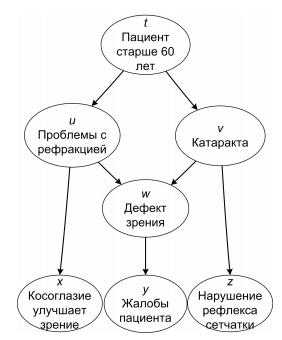
\includegraphics{network}

\url{http://habrahabr.ru/company/surfingbird/blog/176461/}

Суть рассуждений в байсовской сети -- пропагация свидетельств. Обычно пропагация идёт снизу вверх, от следствий к причинам.

\textbf{Теорема о декомпозиции}. Для БСД общее распределение вероятностей $p(X)=p(x_1,\dots,x_n)=\prod\limits_{x\in X}p(x|pa(x))$, где $pa(x)$ -- множество родителей узла $x$ в графе.  

Маргинальные, совместные и условные распределения являются факторами (factor) -- функциями от нескольких переменных. 
Над факторами можно производить некоторые операции: перемножать (multiply), маргинализировать по переменной(marginalize) и уменьшать (reduce). 

\begin{figure}[h!]
    \center{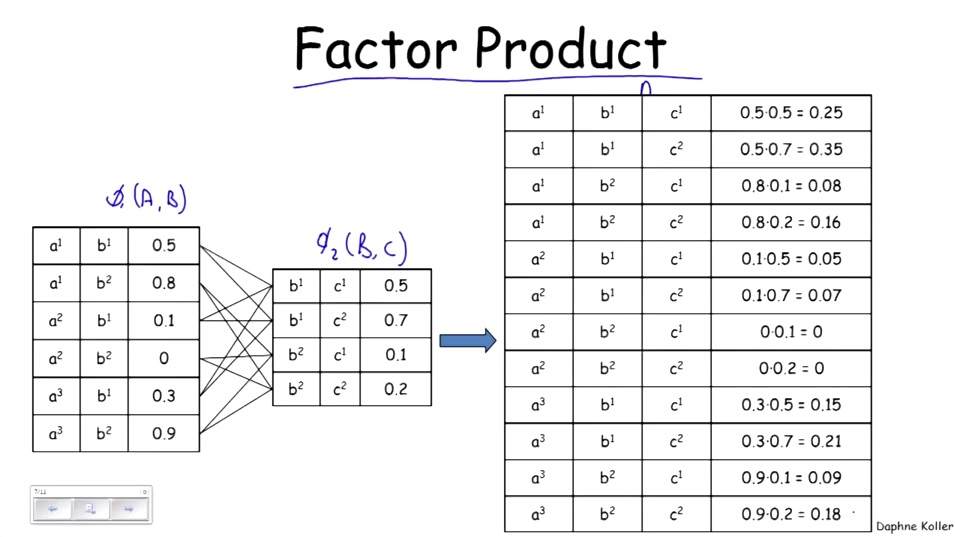
\includegraphics[width=0.8\textwidth]{product}}
    \caption{Произведение факторов}
\end{figure}

\begin{figure}[h!]
    \center{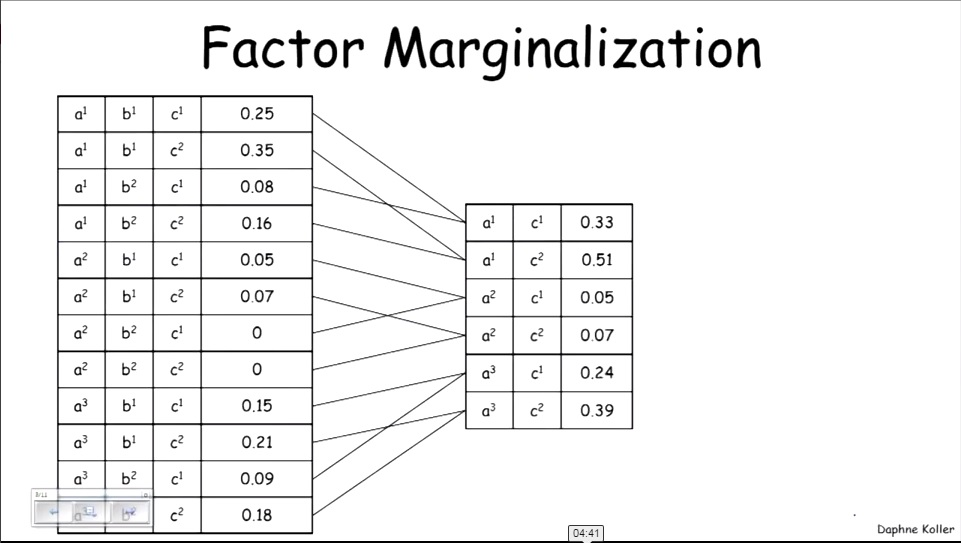
\includegraphics[width=0.8\textwidth]{marginalization}}
    \caption{Маргинализация}
\end{figure}

\begin{figure}[h!]
    \center{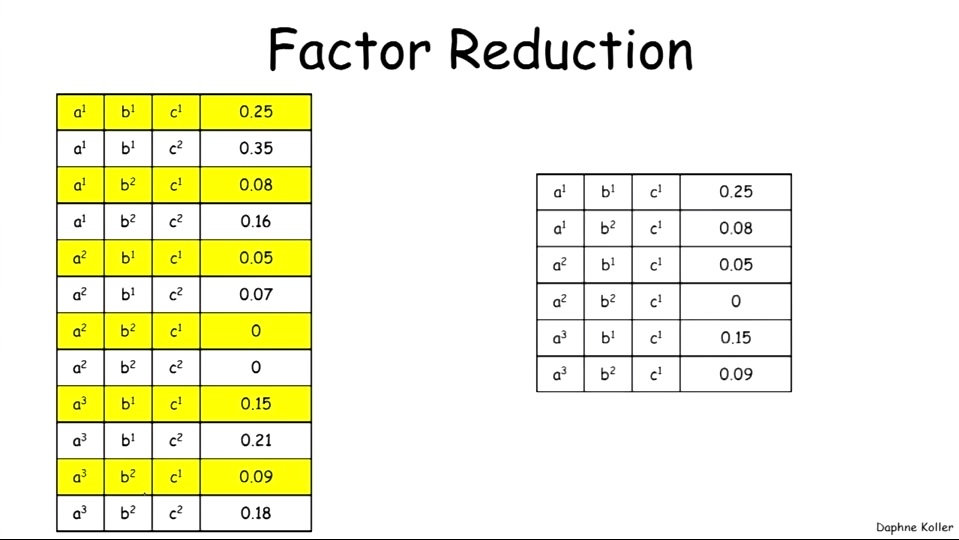
\includegraphics[width=0.8\textwidth]{reduction}}
    \caption{Редукция}
\end{figure}

\subsection{Variable elimination}
Совместное распределение в сети задается через перемножение нескольких факторов, соответствующих вершинам. 
По входным свидетельствам хотим получить апостериорные вероятности событий в сети. 

\begin{enumerate}
    \item Если есть свидетельства, делаем редукцию факторов по ним;
    \item Выбираем событие, содержащееся в наименьшем числе факторов;
    \item Перемножаем и нормируем полученный фактор;
    \item Маргинализуем по выбранному событию;
    \item Если остались события, по которым суммирование еще не делали, возвращаемся на шаг 2.
\end{enumerate}

\begin{figure}[h!]
    \center{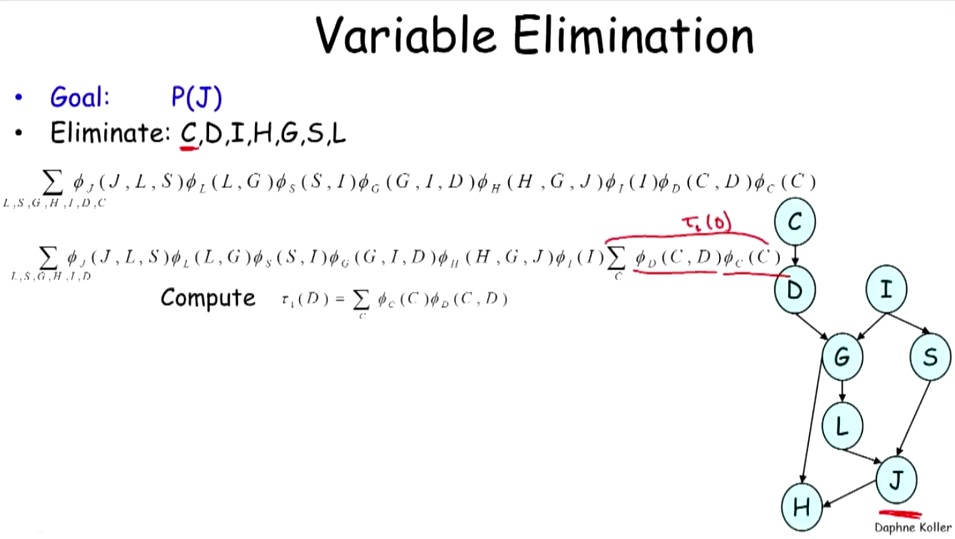
\includegraphics[width=0.8\textwidth]{variable_elimination}}
    \caption{Variable elimination}
\end{figure}

\subsection*{Уменьшение размерности пространства признаков}
\url{http://logic.pdmi.ras.ru/~sergey/teaching/mlauii12/15-pca.pdf}

\textit{Метод главных компонент} -- один из основных способов уменьшить размерность данных, потеряв наименьшее количество информации. 
\begin{enumerate}
    \item Нормируем матрицу $X(d \times n)$ построчно(мат.ожидание 0, дисперсия 1);
    \item Строим матрицу ковариаций $\Sigma=XX^T$;
    \item Вычисляем собственные значения;
    \item Берем собственные вектора, соответстующие k самым большим собственным значениям, и формируем из них матрицу $W$.
    \item Перемножаем полученную матрицу с исходной $Y=WX$. $Y$ имеет размерность $k \times n$ 
\end{enumerate}

Выбирать $k$ можно разными способами:
\begin{itemize}
    \item k = $\sum_i{[\lambda_i>\varepsilon]}$ То есть берем все вектора, собственные значения которых больше $\varepsilon$.
    \item k = $\frac{\sum_{i=1}^k\lambda_i}{\sum_{i=1}^n\lambda_i} > 0.9$
\end{itemize}

Суть метода в нахождении проекции, в которой максимизируется дисперсия и минимизируется суммарное расстояние до проекций точек. 
Оказывется, что необходимо делать проекцию на пространство, базисом в котором являются собственные вектора. 
При этом некоторые вектора (с малым собственным значением) можно отбросить, тем самым уменьшив размерность пространства и потеряв минимум информации. 
PCA позволяет получить матрицу перехода в новое пространство, обнаружить зависимости между признаками исходных данных и сделать некоторый препроцессинг данных (после которого могут быть лучше видны характерные особенности).

\end{document}